\documentclass[10pt] {article}
\usepackage{fourier}
\author{Ankit Goyal \\ankit@cs.utexas.edu \\ Natural Language Processing}
\title{Homework 3: Active Learning for Statistical Parsing}
\date{\today}	
\usepackage{full page}
\usepackage{minted} % to insert code
\renewcommand\listingscaption{Codeblock}


\usepackage{hyperref, url}
\usepackage{listings}
\usepackage{graphicx}
\usepackage{caption}
\usepackage{subcaption}
\usepackage{amsmath}
%\usepackage{amsmath, enumerate, url, ulem, algorithmic, polynom, subfig}
\usepackage{array}
\newcolumntype{L}{>{\centering\arraybackslash}m{2cm}}	

\begin{document}
\maketitle

%----------------------------------------------------------------------------------------
% Introduction begin
%----------------------------------------------------------------------------------------

\section{Introduction}
In this experiment we analyze the performance Active learning methods. For statistical parsing the training instance is sentence and the annotation is the parse tree supplied by a linguist expert. Many learning problems require supervised training however, choosing the appropriate training data may be difficult to obtain. Active learning methods uses uncertainty-based  evaluation functions to estimate the training utility values of a sentence. This selection of training data reduces the size of corpus needed to train without degrading the quality of the induced grammars. \\

\noindent In this homework, we evaluate four different methods to measure uncertainty:	
\begin{itemize}
\item \textbf{Random Selection}: In this evaluation method, in each iteration we simply choose random sentences (with total words >=1500) in each iteration. This doesn't necessarily use any active learning method.
\item \textbf{Sentence Length}: Here as a naive method, we use sentence length as the criteria to measure uncertainty. This function approximates the length with uncertainty. It assumes that longer the sentence, the more uncertain it's parse tree is (which may not always be true).
\item \textbf{Selection Probability}: use the probability assigned to the selected parse tree, the higher the probability, the lower is uncertainty. We choose more uncertain sentences first to better train our parser. we normalize the probabilities by taking $(n-1)th$ root where n is the length of the sentence, since otherwise the long sentences will always be the most uncertain ones.
\item \textbf{Tree Entropy:} as defined by Hwa(2000), we consider top k parses of the sentence as a measure of uncertainty. We use the pseudocode in codeblock 1 to calculate the tree entropy.

%----------------------------------------------------------------------------------------
% Entropy Algorithm begin
%----------------------------------------------------------------------------------------



\begin{listing}[ht!]
\begin{minted}{cpp}
// sum the probability of top 10 parse trees
for (Tree tree : topKparses)
	sum += Math.exp(tree.score());

// normalize the probability of each parse tree.
for (Tree tree: topKparses)
	normalized_scores_list.add(Math.exp(tree.score())/sum)

// calculate entropy as described in Hwa(2000), 
// as expected negative log likelihood of each parse probability.
double entropy = 0.0;
for (double score : normalized_scores_list)
	double ent = -1 * Math.log(score)/Math.log(2) * score
	entropy += ent;

// normalize the entropy with the sentence length.
normalized_entropy = entropy/sentence_length.
\end{minted}
\label{lshed}
\caption{Entropy Calculation}
\end{listing}
\end{itemize}

%----------------------------------------------------------------------------------------
% Entropy Algorithm end
%----------------------------------------------------------------------------------------

%----------------------------------------------------------------------------------------
%Introduction end
%----------------------------------------------------------------------------------------

%----------------------------------------------------------------------------------------
% Experiments begin
%----------------------------------------------------------------------------------------

\section{Experiments:}
\begin{itemize}
\item Section 00 of WSJ corpus was used as a initial data and section 01-03 were used as training data. Section 20 was used for testing.
\item Four selection functions were implemented (random, sentence length, selection probability and tree entropy).
\item F1 score is used to compare different selection functions.
\end{itemize}

\begin{figure}[ht!]
\centering
  %\centering
  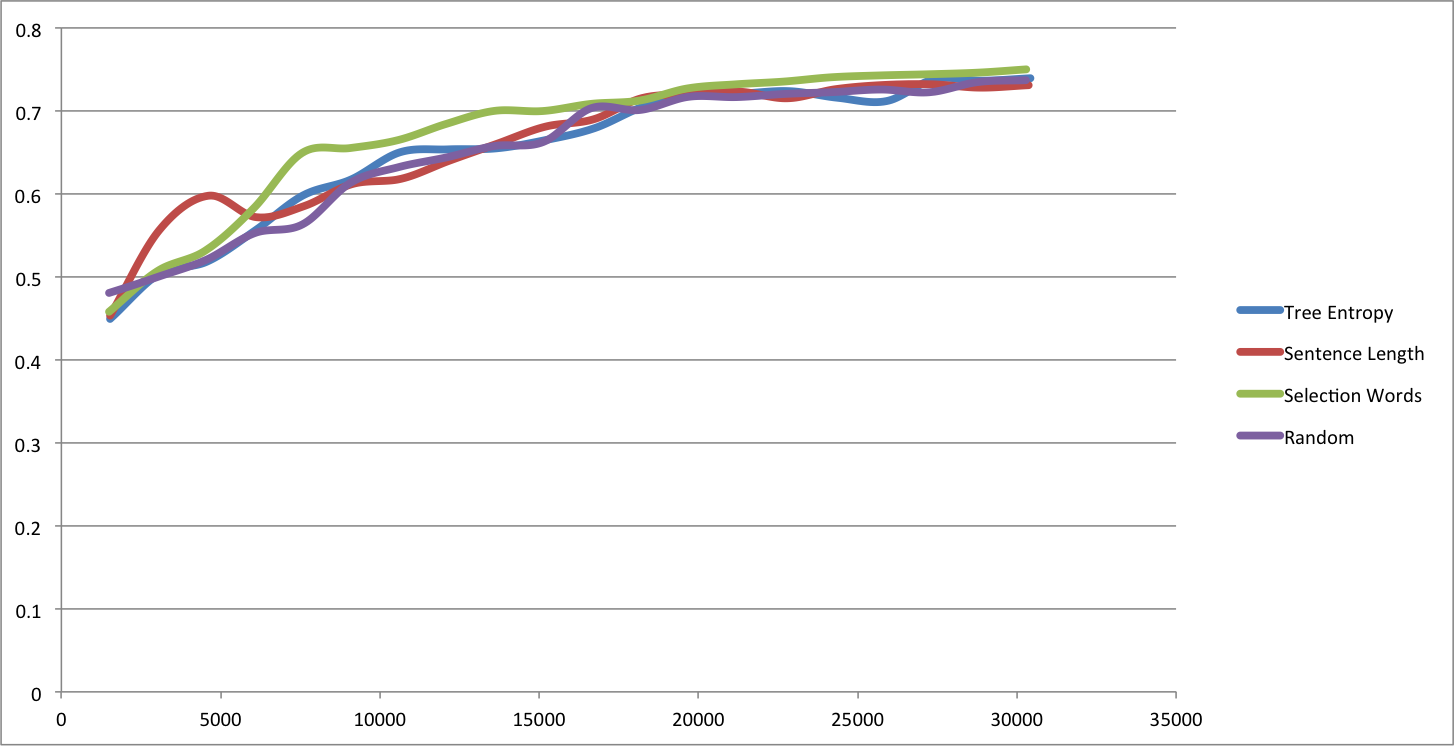
\includegraphics[width=\linewidth]{chart.png}
  \caption{F1 vs Number of training words}
  \label{fig:thvsfair}
\end{figure}

%----------------------------------------------------------------------------------------
% Experiments end
%----------------------------------------------------------------------------------------

%----------------------------------------------------------------------------------------
% Observations begin
%----------------------------------------------------------------------------------------


\section{Observations:}

\begin{enumerate}
\item Active learning methods does seem to perform better than random selection since we are training on more complex data by actively selecting to train our parser better.
\item Tree entropy doesn't perform as well as expected or as it is mentioned in the paper. One of the reasons for this could be the dataset. 
\item Selective probability performs the best and random performs the worst (very close to selection by length). The difference is performance of tree entropy and sentence length or random selection is not as huge as mentioned in the paper.
\end{enumerate}

%----------------------------------------------------------------------------------------
% Observations End
%----------------------------------------------------------------------------------------

%----------------------------------------------------------------------------------------
% References Begin
%----------------------------------------------------------------------------------------


\section{References:}
\begin{enumerate}
\item Rebecca Hwa. Sample Selection for Statistical Grammar Induction. 
\end{enumerate}

%----------------------------------------------------------------------------------------
% References End
%----------------------------------------------------------------------------------------



\end{document}